\documentclass{article}%
\usepackage[T1]{fontenc}%
\usepackage[utf8]{inputenc}%
\usepackage{lmodern}%
\usepackage{textcomp}%
\usepackage{lastpage}%
\usepackage{authblk}%
\usepackage{graphicx}%
%
\title{Upregulation of PIAS1 protects against sodium taurocholate{-}induced severe acute pancreatitis associated with acute lung injury}%
\author{Gabriel Bartlett}%
\affil{Department of Developmental, Molecular and Chemical Biology, Tufts University School of Medicine, Boston, Massachusetts, United States of America}%
\date{01{-}01{-}2014}%
%
\begin{document}%
\normalsize%
\maketitle%
\section{Abstract}%
\label{sec:Abstract}%
Please enable Javascript to watch this video\newline%
Cepharanthine hydrochloride is being used in the treatment of a rare blood disease which the symptoms mimic AML (Ampliciti{-}Mutant Haemophilia).\newline%
Researchers at the University of Southern California tested a different regimen for AML patients and found that they could live longer than those that were given the Cepharanthine regimen alone.\newline%
Since trials with the patient have been stopped because of safety concerns, researchers are going back to normal therapy in those patients to see if they have any lingering effects from the Cepharanthine use.\newline%
Another LA team tested a cholesterol drug which only contains angiotensin II receptor blockers which allows the enzyme of AML to be used to speed up the metabolism of cholesterol rather than suppressing it.\newline%
A CYP2D6 gene from patients with AML was switched off or restored through a failed drug cocktail that brought it back on. The team found that the cancer came back or developed faster when the same drugs were used on patients with AML.\newline%
The study doesn't show what happens in the relapsing patients, however. Some patients in this group showed "reduced" exposure to Cepharanthine because they were not injected or sedated.

%
\subsection{Image Analysis}%
\label{subsec:ImageAnalysis}%


\begin{figure}[h!]%
\centering%
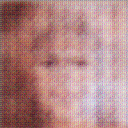
\includegraphics[width=150px]{500_fake_images/samples_5_186.png}%
\caption{A Close Up Of A Person Holding A Toothbrush}%
\end{figure}

%
\end{document}